\documentclass{beamer}

\usepackage{graphicx}
\usepackage{mathtools}
\usepackage{mathrsfs}

%Information to be included in the title page:
\title{Assumptions for Causal Inference}
\author{Congyuan Duan}
%\institute{School of Mathematics, Sun Yat-sen University}



\begin{document}

\frame{\titlepage}

\begin{frame}
    \frametitle{Contents}
    \tableofcontents
\end{frame}

\section{Example}

\begin{frame}
    \frametitle{Contents}
    \tableofcontents[currentsection]
\end{frame}

\begin{frame}
    \frametitle{Example}
    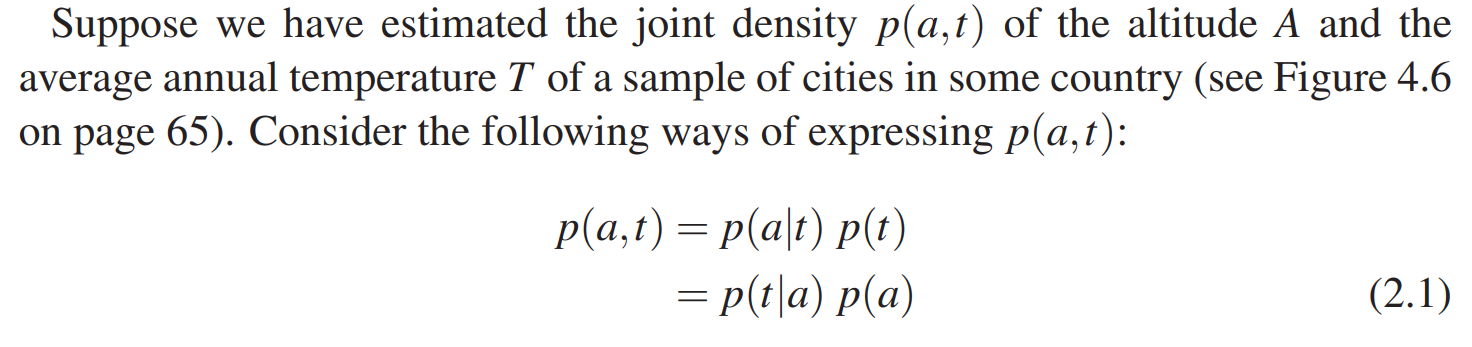
\includegraphics[scale=0.6]{fig3.png}
    How to decide which of the two structures is the causal one? 
\end{frame}

\begin{frame}
    \frametitle{Example}

    \begin{itemize}
        \item[$\bullet$] Effect of interventions
        \item[$\bullet$] Independence of cause and mechanism 
        \item[$\bullet$] Independent noises
    \end{itemize}
\end{frame}

\section{Independent Mechanisms}

\begin{frame}
    \frametitle{Contents}
    \tableofcontents[currentsection]
\end{frame}

\begin{frame}
    \frametitle{Principle}
    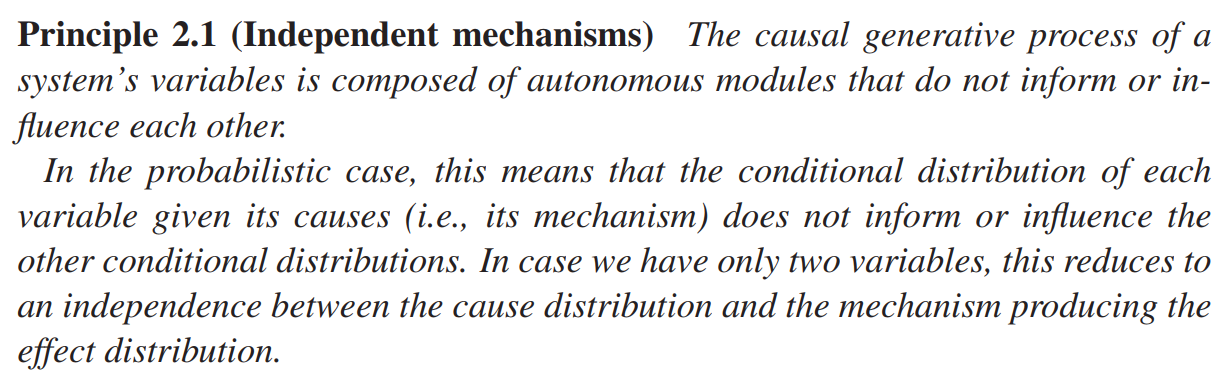
\includegraphics[scale=0.6]{fig1.png}
    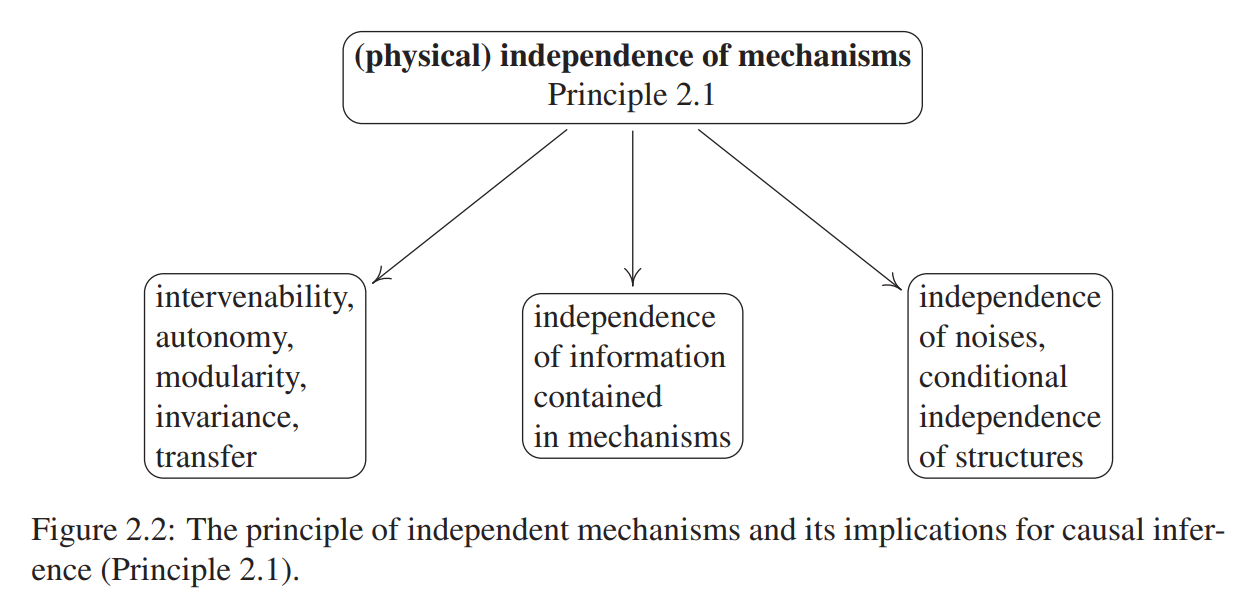
\includegraphics[scale=0.6]{fig2.png}
\end{frame}




\end{document}
